%\RequirePackage[ngerman=ngerman-x-latest]{hyphsubst}

\documentclass[	
	british,
	cdgeometry=true, % Setting the type area
	headingsvskip=-2.5cm, % Moving the title (\title{}\maketitle) in vertical direction
	cdhead=nocolor, %color scheme Kopfzeile: nocolor, lightcolor, barcolor, bicolor
	cdhead=nodate, %Print date right-aligned in header: date, nodate
	cdfont=true,
	ddc=false, %Dresden concept logo: false, true, color, colorblack, gray, black, blue, white
	parskip=true,
	titlepage=true
]{tudscrartcl}

\usepackage{selinput}\SelectInputMappings{adieresis={ä},germandbls={ß}}
\usepackage[default, osfigures]{opensans}
\usepackage[T1]{fontenc}
\usepackage{babel}
\usepackage{blindtext}
\usepackage{amsmath}
\usepackage{empheq}
\usepackage{booktabs}
\usepackage[version=4]{mhchem}
\usepackage[decimalsymbol=comma,loctolang={DE:ngerman,UK:english}]{siunitx}
\usepackage{amssymb}
\usepackage{listings} %Quellcode einbinden!
\usepackage{enumitem}
\usepackage{acronym}

\newcommand{\lsttxt}[1]{\textbf{\lstinline|#1|}}

\begin{document}

\lstset{language=Matlab}
\setlist[itemize]{partopsep=0pt,parsep=5pt}

% Head
\faculty{School of Engineering}
\institute{Chair of Process Control Systems \& Process Systems Engineering Group}
%\faculty{Faculty Mechanical Engineering}
%\institute{Institute for Process Engineering and Environmental Technology}
%\chair{WG System Process Engineering}
%\extraheadline{}
\headlogo[height=2cm]{images/PLT_Logo_RGB.png} % Integration of the PLT/SVT logo

% Dokumententitel
\title{Projectreport\\
		Mensch-Maschine-Systemtechnik\\
		Winter term 2021-2022\vspace{20mm}
		}
		
%\vspace{10mm}
\newcommand{\Gruppennummer}{10}
\newcommand{\Gruppentitel}{asd}

\subtitle{Group: \Gruppennummer\space-\space\Gruppentitel \vspace{20mm}}

\date{Start of editing: \hspace{15mm} XX.YY.2021 \\
		  Submission day: \hspace{13.5mm} XX.YY.2022}

\author{Felix Mehlhorn
	\and
	Marcus Rothhaupt
	\and
	Artan Kabashi
	\and
	Dmytro Kostiuk
	\and
	Tamino Schorcht}
	
\maketitle

%% Document title Ende

\tableofcontents
\newpage

%% List of abbreviations and symbols

\section*{List of abbreviations and symbols}
\addcontentsline{toc}{section}{List of abbreviations and symbols}

\subsection*{List of symbols}
\addcontentsline{toc}{subsection}{List of symbols}
	\begin{acronym}[MMST1]
		\acro{MMST1}[MMST]{Mensch-Maschine-Systemtechnik}
	\end{acronym}
\subsection*{List of abbreviations}
\addcontentsline{toc}{subsection}{List of abbreviations}
	\begin{acronym}[MMST2]
		\acro{MMST2}[MMST]{Mensch-Maschine-Systemtechnik}
	\end{acronym}
\newpage

%% Task description

\section*{Task Description}
\addcontentsline{toc}{section}{Task Description}

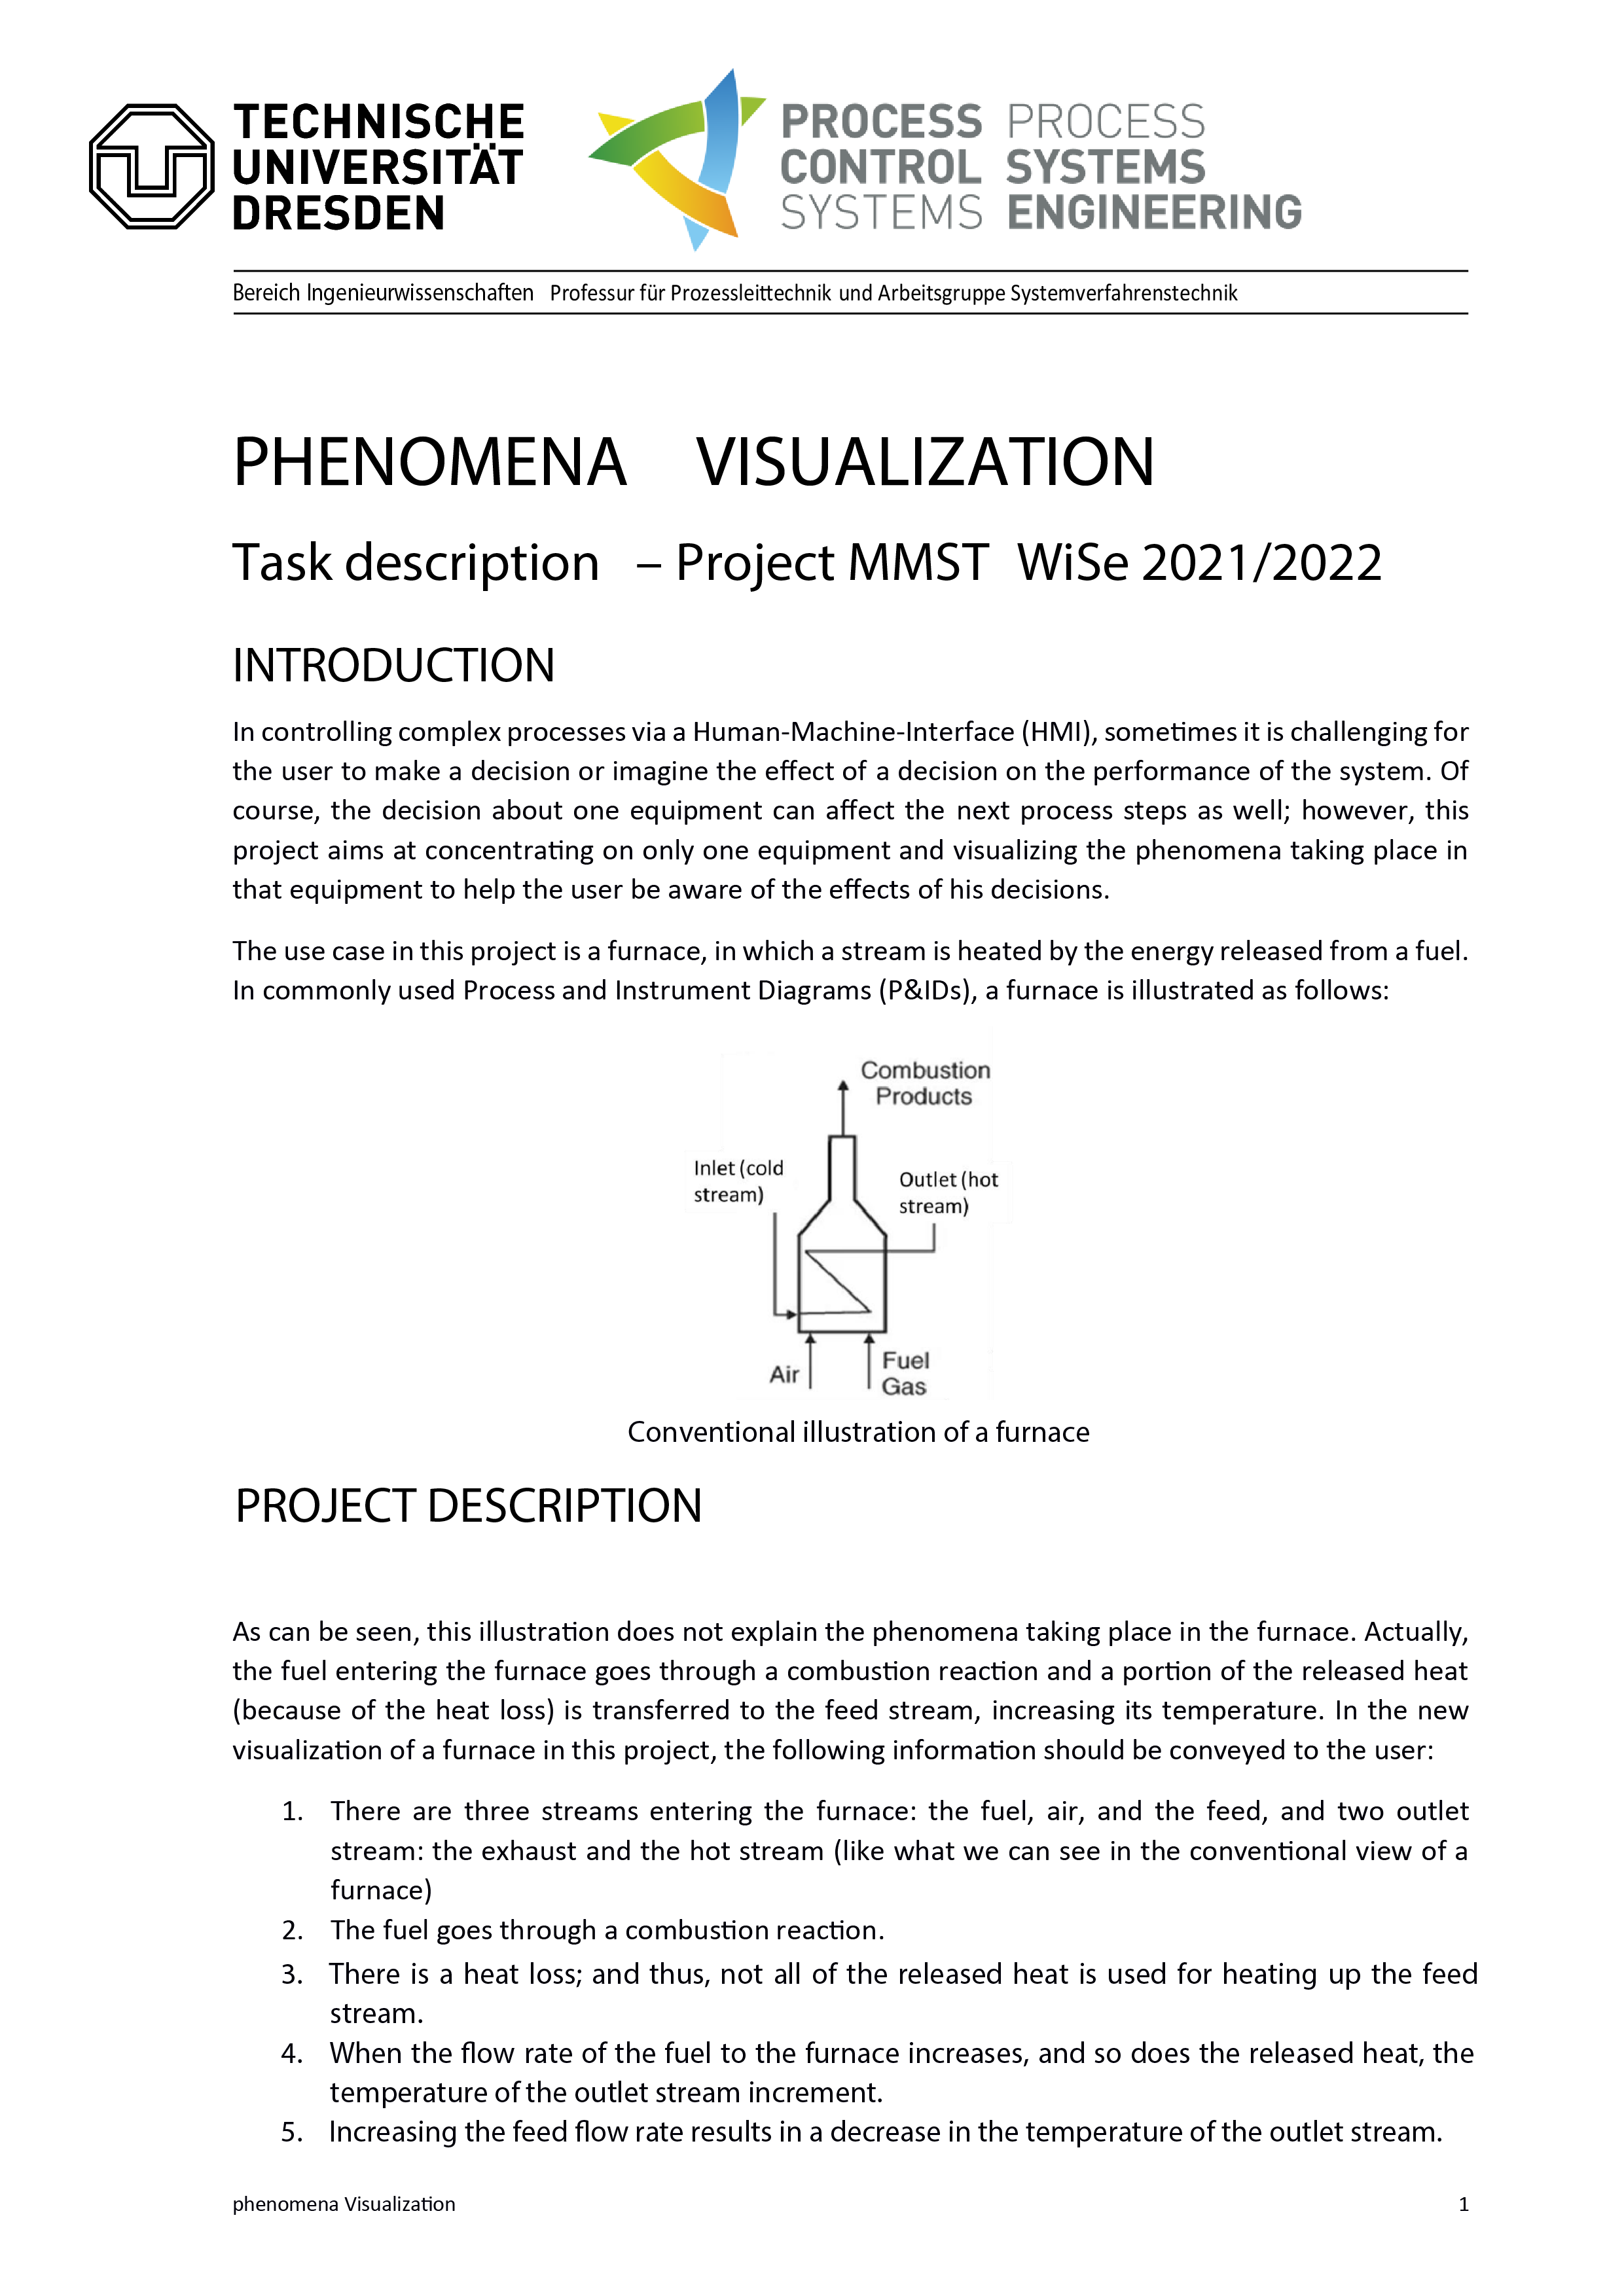
\includegraphics[page=1,scale=0.72]{images/MMST_Aufgabenstellung_PhenomenaVisualization.png}
\newpage

%% Introduction

\section*{Introduction}

The human can often be the deciding factor if a process works correctly or not. It can be diffucult to  estimate the outcome certain interactions between human and machine cause. Therefore it is important for the Operator to understand the process he or she is working on.
\newline
This article focuses on visualizing the phenomena happening in a furnace, to give the user an understanding of the system and consequently reduce mistakes, potentially made by an operator.
\newline
The furnace, whom is looked at in this project, has 3 inputs (inlet, air and fuel) and 2 ouputs (outlet and combustion products). The stream gets heated by the energy released from the fuel. It is a simple model and serves as concept to show our tools used to make a process understandable.
\newline

\addcontentsline{toc}{section}{Introduction}

\newpage

%% Requirements

\section*{Requirements}
\addcontentsline{toc}{section}{Requirements}
\newpage

%% Concept

\section*{Concept}
\addcontentsline{toc}{section}{Concept}
\newpage

%% Implementation

\section*{Implementation}
\addcontentsline{toc}{section}{Implementation}
\newpage

%% Validation

\section*{Validation}
\addcontentsline{toc}{section}{Validation}
\newpage

%% Summary

\section*{Summary}
\addcontentsline{toc}{section}{Summary}
\newpage

Random citation \cite{DUMMY:1} embeddeed in text.

\bibliography{bibliography.bib}
\bibliographystyle{ieeetr}
\addcontentsline{toc}{section}{References}

\end{document}